% Extracted from LaTeX-examples-master/tikz/thales-circle-triangle.
% The original tkzDrawSector call is deliberately outside this line-circle slice.
\documentclass[border=2pt]{standalone}
\usepackage{tikz}
\usepackage{tkz-euclide}
\usetikzlibrary{calc}
\begin{document}
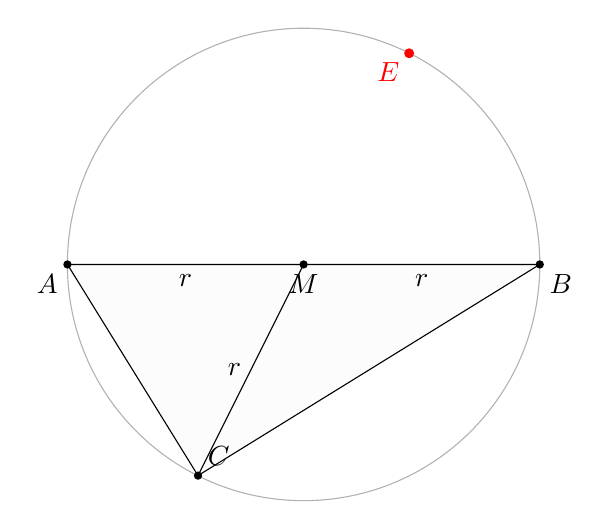
\begin{tikzpicture}[scale=1.5]
  \tkzDefPoint(0,0){A}
  \tkzDefPoint(4,0){B}
  \tkzDefPoint(2,0){M}
  \tkzDefPoint(3,2){H}

  \tkzInterLC[/tikz/overlay](M,H)(M,B) \tkzGetPoints{E}{C}

  \draw[color=gray!60] (M) circle (2cm);
  \draw[rounded corners=0.1mm,fill=gray!2] (A) -- (B) -- (C) -- cycle;
  \draw (M) -- (C);
  \fill (A) circle (1pt) (B) circle (1pt) (M) circle (1pt) (C) circle (1pt);
  \fill[red] (E) circle (1.2pt);
  \node[below left] at (A) {$A$};
  \node[below right] at (B) {$B$};
  \node[below] at (M) {$M$};
  \node[above right] at (C) {$C$};
  \node[below left,red] at (E) {$E$};
  \node[below] at ($(A)!.5!(M)$) {$r$};
  \node[below] at ($(M)!.5!(B)$) {$r$};
  \node[left] at ($(M)!.5!(C)$) {$r$};
\end{tikzpicture}
\end{document}
